\documentclass[10pt,landscape]{article}
\usepackage{multicol}
\usepackage{calc}
\usepackage{ifthen}
\usepackage[landscape]{geometry}
\usepackage{amssymb}
\usepackage{amsmath}
\usepackage{galois}
\usepackage{graphicx}

% To make this come out properly in landscape mode, do one of the following
% 1.
%  pdflatex latexsheet.tex
%
% 2.
%  latex latexsheet.tex
%  dvips -P pdf  -t landscape latexsheet.dvi
%  ps2pdf latexsheet.ps


% If you're reading this, be prepared for confusion.  Making this was
% a learning experience for me, and it shows.  Much of the placement
% was hacked in; if you make it better, let me know...


% 2008-04
% Changed page margin code to use the geometry package. Also added code for
% conditional page margins, depending on paper size. Thanks to Uwe Ziegenhagen
% for the suggestions.

% 2006-08
% Made changes based on suggestions from Gene Cooperman. <gene at ccs.neu.edu>


% To Do:
% \listoffigures \listoftables
% \setcounter{secnumdepth}{0}


% This sets page margins to .5 inch if using letter paper, and to 1cm
% if using A4 paper. (This probably isn't strictly necessary.)
% If using another size paper, use default 1cm margins.
\ifthenelse{\lengthtest { \paperwidth = 11in}}
	{ \geometry{top=1cm,left=1cm,right=1cm,bottom=1cm} }
	{\ifthenelse{ \lengthtest{ \paperwidth = 297mm}}
		{\geometry{top=1cm,left=1cm,right=1cm,bottom=1cm} }
		{\geometry{top=1cm,left=1cm,right=1cm,bottom=1cm} }
	}

% Turn off header and footer
\pagestyle{empty}
 

% Redefine section commands to use less space
\makeatletter
\renewcommand{\section}{\@startsection{section}{1}{0mm}%
                                {-1ex plus -.5ex minus -.2ex}%
                                {0.5ex plus .2ex}%x
                                {\normalfont\large\bfseries}}
\renewcommand{\subsection}{\@startsection{subsection}{2}{0mm}%
                                {-1explus -.5ex minus -.2ex}%
                                {0.5ex plus .2ex}%
                                {\normalfont\normalsize\bfseries}}
\renewcommand{\subsubsection}{\@startsection{subsubsection}{3}{0mm}%
                                {-1ex plus -.5ex minus -.2ex}%
                                {1ex plus .2ex}%
                                {\normalfont\small\bfseries}}
\makeatother

% Define BibTeX command
\def\BibTeX{{\rm B\kern-.05em{\sc i\kern-.025em b}\kern-.08em
    T\kern-.1667em\lower.7ex\hbox{E}\kern-.125emX}}

% Don't print section numbers
\setcounter{secnumdepth}{0}


\setlength{\parindent}{0pt}
\setlength{\parskip}{0pt plus 0.5ex}


% -----------------------------------------------------------------------

\begin{document}

\raggedright
\footnotesize
\begin{multicols}{3}


% multicol parameters
% These lengths are set only within the two main columns
%\setlength{\columnseprule}{0.25pt}
\setlength{\premulticols}{1pt}
\setlength{\postmulticols}{1pt}
\setlength{\multicolsep}{1pt}
\setlength{\columnsep}{2pt}

\begin{center}
  \Large{Abstract interpretation} \\
  \normalsize{Mathematical Tools}\\
  \vspace{0.3cm}
  \tiny {Inspir\'{e} des notes de cours du MPRI d'Antoine Min\'{e}, CNRS/ENS Ulm}\\
\end{center}

\section{Introduction}

\subsection{Concrete semantics}

\begin{eqnarray*}
\mathcal{S}_i \in \mathcal{D} = \mathcal{P} (\{ \verb!I!, \verb!X! \} \rightarrow \mathbb{Z})
\end{eqnarray*}

\begin{tabular}{@{}lll@{}}
$(\mathcal{S}_0)$ \verb!assume X in [0, 1000];! & $\mathcal{S}_0 $ & $= \{ (i, x) : i, x \in \mathbb{Z}\}$\\
                                                &                  & $= \top$\\
$(\mathcal{S}_1)$ \verb!I := 0!  & $\mathcal{S}_1 $ & $= \{ (i, x) \in \mathcal{S}_0: x \in [0, 1000] \} $\\
                                                &                  & $= F_1(\mathcal{S}_0)$\\
$(\mathcal{S}_2)$ & $\mathcal{S}_2 $ & $= \{ (0, x) : \exists i, (i, x) \in \mathcal{S}_1 \} $\\
                                                &                  & $= F_2(\mathcal{S}_1)$\\
\verb!while! $(\mathcal{S}_3)$ \verb!I < X do! & $\mathcal{S}_3 $ & $= \mathcal{S}_2 \cup \mathcal{S}_5$ \\
\verb!  !$(\mathcal{S}_4)$\verb!I := I + 2;!  & $\mathcal{S}_4 $ & $= \{ (i, x) \in \mathcal{S}_3 : i < x\} $ \\
                                                &                  & $= F_4(\mathcal{S}_3)$\\
\verb!  !$(\mathcal{S}_5)$ & $\mathcal{S}_5 $ & $= \{ (i + 2, x) : (i, x) \in \mathcal{S}_4 $\\
                                                &                  & $= F_5(\mathcal{S}_4)$\\
$(\mathcal{S}_6)$ & $\mathcal{S}_6 $ & $= \{ (i, x) \in \mathcal{S}_3 : i \geq x \} $\\
                                                &                  & $= F_6(\mathcal{S}_3)$
\end{tabular}

\begin{itemize}\setlength{\itemsep}{-0.7mm}
\item smallest solution of a system of equations
\item strongest invariant (and an inductive invariant)
\item not computable in general
\end{itemize}

\subsection{Abstract semantics}

\begin{eqnarray*}
\mathcal{S}_i^{\sharp} \in \mathcal{D}^{\sharp}
\end{eqnarray*}

\begin{tabular}{@{}ll@{}}
$(\mathcal{S}_0)$ \verb!assume X in [0, 1000];! & $\mathcal{S}_0^{\sharp} = \top^{\sharp}$\\
$(\mathcal{S}_1)$ \verb!I := 0!  & $\mathcal{S}_1^{\sharp} = F_1^{\sharp} (\mathcal{S}_0^{\sharp})$\\
$(\mathcal{S}_2)$ & $\mathcal{S}_2^{\sharp} = F_2^{\sharp} (\mathcal{S}_1^{\sharp})$\\
\verb!while! $(\mathcal{S}_3)$ \verb!I < X do! & $\mathcal{S}_3^{\sharp} = \mathcal{S}_2^{\sharp} \cup^{\sharp} \mathcal{S}_5^{\sharp}$\\
\verb!  !$(\mathcal{S}_4)$\verb!I := I + 2;!  & $\mathcal{S}_4^{\sharp} = F_4^{\sharp} (\mathcal{S}_3^{\sharp})$ \\
\verb!  !$(\mathcal{S}_5)$ & $\mathcal{S}_5^{\sharp} = F_5^{\sharp} (\mathcal{S}_4^{\sharp})$\\
$(\mathcal{S}_6)$ & $\mathcal{S}_6^{\sharp} = F_6^{\sharp} (\mathcal{S}_3^{\sharp})$
\end{tabular}

\begin{itemize}\setlength{\itemsep}{-0.7mm}
\item $\mathcal{D}^{\sharp}$ subset of properties of interest (with a machine repr.))
\item $F^{\sharp} : \mathcal{D}^{\sharp} \rightarrow \mathcal{D}^{\sharp}$ over-approximates the effect of $F : \mathcal{D} \rightarrow \mathcal{D}$ in $\mathcal{D}^{\sharp}$ (with effective algorithms).
\end{itemize}

\subsection{Numeric abstract domain examples}

%% TODO image
\begin{center}
  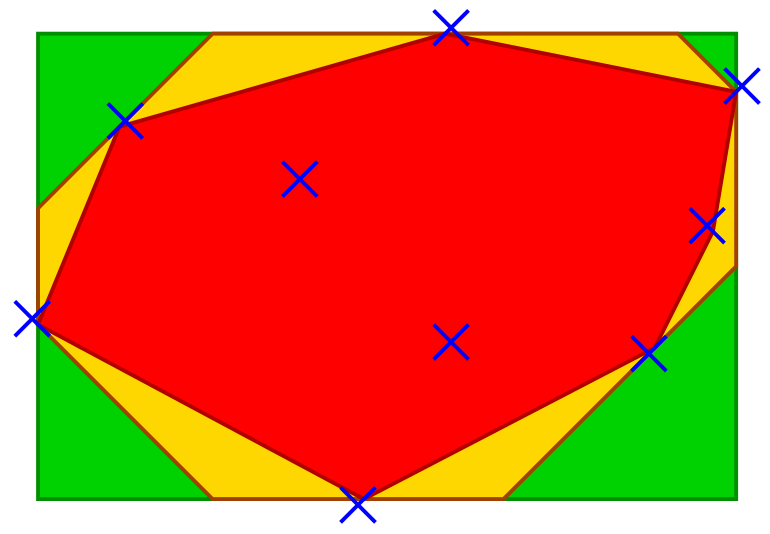
\includegraphics[height=100px]{figures/numerical_domains_examples.png}
\end{center}

\begin{tabular}{@{}lll@{}}
concrete sets $\mathcal{D}$           & $\{ (0, 3), (5.5, 0), (12, 7), \dots\}$       & not comp.\\
abs. polyhedra $\mathcal{D}^{\sharp}_p$ & $6X + 11Y \geq 33 \wedge \dots$               & exp. cost\\
abs. octogons $\mathcal{D}^{\sharp}_o$  & $X + Y \geq 3 \wedge Y \wedge 0 \wedge \dots$ & cubic cost\\
abs. intervals $\mathcal{D}^{\sharp}_i$ & $X \in [0, 12] \wedge Y \in [0, 8]$           & linear cost
\end{tabular}

Trade-off between cost and expressiveness/precision.

%\subsection{Correctness proof and false alarms}

%% TODO image 2
%\begin{center}
%  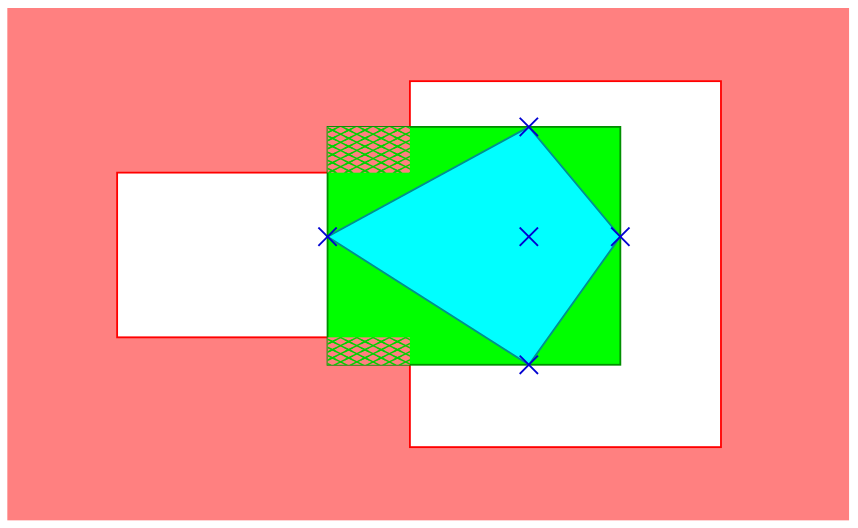
\includegraphics[height=100px]{figures/false_alarms.png}
%\end{center}

%Program is correct (blue $\cap$ red $= \varnothing$). The polyhedra domain \textbf{can} prove the correctness (cyan $\cap$ red $= \varnothing$). The interval domain \textbf{cannot} (green $\cap$ red $\neq \varnothing$, false alarm).

\subsection{Galois connection}
\begin{eqnarray*}
(\mathcal{D}, \subseteq) &\galois{\alpha}{\gamma}& (\mathcal{D}^{\sharp}, \subseteq^{\sharp})\\
\alpha (X) \subseteq^{\sharp} Y^{\sharp} &\Leftrightarrow& X \subseteq \gamma (Y^{\sharp})
\end{eqnarray*}

\begin{itemize}\setlength{\itemsep}{-0.7mm}
\item $\alpha(X)$ is the best abstraction of $X$ in $\mathcal{D}^{\sharp}$
\item $F^{\sharp} = \alpha \circ F \circ \gamma$ is the best abstraction of $F$ in $\mathcal{D}^{\sharp} \rightarrow \mathcal{D}^{\sharp}$
\end{itemize}

\textbf{Example.} (interval domain $\mathcal{D}^{\sharp}_i$)
\begin{itemize}\setlength{\itemsep}{-0.7mm}
\item $[l_1, h_1] \subseteq^{\sharp}_i [l_2, h_2] \Leftrightarrow l_1 \geq l2 \wedge h_1 \leq h_2$
\item $\gamma_i([l, h]) = \{ x \in \mathbb{Z} : l \leq x \leq h\}$
\item $\alpha_i (X) = [\operatorname {min} X, \operatorname {max} X]$
\end{itemize}

\subsection{Resolution by iteration and extrapolation}

\textbf{Problem.} the equation system is recursive : $\overrightarrow{\mathcal{S}}^{\sharp} = \overrightarrow{F}^{\sharp} (\overrightarrow{\mathcal{S}}^{\sharp})$

\textbf{Solution.} resolution by iteration : $\overrightarrow{\mathcal{S}}^{\sharp 0} = \varnothing^{\sharp}$, $\overrightarrow{\mathcal{S}}^{\sharp i + 1} = \overrightarrow{F}^{\sharp} (\overrightarrow{\mathcal{S}}^{\sharp i})$

e.g. $\mathcal{S}_3^{\wedge}$ : $\verb!I! \in \varnothing$, $\verb!I! = 0$, $\verb!I! \in [0, 2]$, $\verb!I! \in [0, 4]$, $\dots$, $\verb!I! \in [0, 1000]$

\textbf{Problem.} infinite or very long sequence of iterate in $\mathcal{D}^{\sharp}$

\textbf{Solution.} extrapolation operator $\bigtriangledown$

e.g. $[0, 2] \bigtriangledown [0, 4] = [0, +\infty[$

\begin{itemize}\setlength{\itemsep}{-0.7mm}
\item remove unstable bounds and constraits
\item ensures the convergence in finite time
\item inductive reasoning (through generalisation)
\end{itemize}

\section{Order theory}

\textbf{Definition.} Set $X$. $\sqsubseteq \in X \times X$ is a \textbf{partial order} iff
\begin{enumerate}\setlength{\itemsep}{-0.7mm}
\item reflexive: $\forall x \in X, x \sqsubseteq x$
\item antisymmetric: $\forall x, y \in X, x \sqsubseteq y \wedge y \sqsubseteq x \Rightarrow x = y$
\item transitive: $\forall x, y, z \in X, x \sqsubseteq y \wedge y \sqsubseteq x \wedge y \sqsubseteq z \Rightarrow x \sqsubseteq z$
\end{enumerate}

$(X, \sqsubseteq)$ is a \textbf{poset} (partially ordered set).

Without antisymmetry, $\sqsubseteq$ is a \textbf{preorder}.

\textbf{Examples.} $(\mathbb{Z}, \leq)$, $(\mathcal{P}(X), \subseteq)$, $\forall S, (S, =)$.

\textbf{Usage.}
\begin{itemize}\setlength{\itemsep}{-0.7mm}
\item logic: ordered by implication $\Rightarrow$
\item approximations: $\sqsubseteq$ is an information order
\item program verification: program semantics $\sqsubseteq$ specification
\end{itemize}

\textbf{Definitions.}
\begin{itemize}\setlength{\itemsep}{-0.7mm}
\item $c$ is an \textbf{upper bound of $a$ and $b$} if $a \sqsubseteq c$ and $b \sqsubseteq c$
\item { $c$ is an \textbf{least upper bound of $a$ and $b$} (\textbf{lub} or \textbf{join}) if
  \begin{itemize}\setlength{\itemsep}{-0.7mm}
  \item $c$ is and upper bound of $a$ and $b$
  \item for every upper bound $d$ of $a$ and $b$, $c \sqsubseteq d$
  \end{itemize}
  Unique and noted $a \sqcup b$.
}
\end{itemize}

Generalized to upper bounds of arbitrary sets : $\sqcup Y$, $Y \subseteq X$.

$a \sqcap b$, $\sqcap Y$ are \textbf{greatest lower bounds} (\textbf{glb} or \textbf{meet}) if $a \sqcap b \sqsubseteq a, b$ and $\forall c, c \sqsubseteq a, b \Rightarrow c \sqsubseteq a \sqcap b$.

$C \subseteq X$ is a \textbf{chain in $(X, \sqsubseteq)$} if it is totally ordered : $\forall x, y \in C, x \sqsubseteq y \vee y \sqsubseteq x$.

Poset $(X, \sqsubseteq)$ is a \textbf{complete partial order} (\textbf{CPO}) if every chain $C$ (incl. $\varnothing$) has a least upper bound $\sqcup C$.

A CPO has a \textbf{least element} $\sqcup \varnothing$, denoted $\perp$.

\textbf{Examples.}
\begin{itemize}\setlength{\itemsep}{-0.7mm}
\item $(\mathbb{N}, \leq)$ not complete, $(\mathbb{N} \cup \{ \infty \}, \leq)$ compl.
\item $(\{ x \in \mathbb{Q} : 0 \leq x \leq 1\}, \leq)$ not compl. but $(\{ x \in \mathbb{R} : 0 \leq x \leq 1\}, \leq)$ compl.
\item $\forall Y, (\mathcal{P}(Y), \subseteq)$ compl.
\end{itemize}

\textbf{Definition.} Poset $(X, \sqsubseteq, \sqcup, \sqcap)$ is a \textbf{lattice} with
\begin{enumerate}\setlength{\itemsep}{-0.7mm}
\item a lub $a \sqcup b$ for every pair of $a$ and $b$
\item a glb $a \sqcap b$ for every pair of $a$ and $b$
\end{enumerate}

\textbf{Examples.}
\begin{itemize}\setlength{\itemsep}{-0.7mm}
\item integer intervals: $(\{ [a, b] : a, b \in \mathbb{Z}, a \leq b\} \cup \{ \varnothing \}, \subseteq, \sqcup, \cap)$ where $[a, b] \sqcup [c, d] = [\operatorname{min} (a, a'), \operatorname{max} (b, b')]$.
\item divisibility: $(\mathbb{N}^{\star}, |, \operatorname{gcd}, \operatorname{lcm})$
\end{itemize}

\textbf{Definition.} Poset $(X, \sqsubseteq, \sqcup, \sqcap, \perp, \top)$ is a \textbf{complete lattice} with
\begin{enumerate}\setlength{\itemsep}{-0.7mm}
\item a lub $\sqcup S$ for every set $S \subseteq X$
\item a glb $\sqcap S$ for every set $S \subseteq X$
\item a least element $\perp$
\item a greatest element $\top$
\end{enumerate}

\textbf{Examples.}
\begin{itemize}\setlength{\itemsep}{-0.7mm}
\item real segment $[0, 1]$: $([0, 1], \leq, \operatorname{max}, \operatorname{min})$
\item powersets: $(\mathcal{P}(S), \subseteq, \cup, \cap, \varnothing, S)$
\item finite lattices
\item integer intervals with finite and infinite bounds
\end{itemize}

\subsection{Derivation}

Complete posets or lattices $(X, \sqsubseteq_X, \dots)$ and $(Y, \sqsubseteq_Y, \dots)$, we can derive new ones by: duality, adding a least element $\perp$ (lifting), product, point-wise lifting by some set $S$, sublattice.

\subsection{Fixpoints}

\textbf{Definition.} A function $f : (X, \sqsubseteq_X, \dots) \rightarrow (Y, \sqsubseteq_Y, \dots)$ is
\begin{itemize}\setlength{\itemsep}{-0.7mm}
\item \textbf{monotonic} if $\forall x, x', x \sqsubseteq_X x' \Rightarrow f(x) \sqsubseteq_Y f(x')$
\item \textbf{strict} if $f (\perp_X) = \perp_Y$
\item \textbf{continuous between CPOs} if $C \operatorname{chain} \subseteq X, \{ f(c) : c \in C \}$ is a chain in $Y$ and $f (\sqcup_X C) = \sqcup_Y \{ f(c) : c \in C\}$
\item a \textbf{complete $\sqcup -$morphism between complete lattices} if $\forall S \subseteq X, f (\sqcup_X S) = \sqcup_Y \{ f(s) : s \in S \}$
\item \textbf{extensive} if $X = Y$ and $\forall x, x \sqsubseteq_X f(x)$
\end{itemize}

\textbf{Definition.} Given $f : (X, \sqsubseteq) \rightarrow (X, \sqsubseteq)$
\begin{itemize}\setlength{\itemsep}{-0.7mm}
\item $x$ is a \textbf{fixpoint} of $f$ if $f(x) = x$
\item $x$ is a \textbf{prefixpoint} of $f$ if $x \sqsubseteq f(x)$
\item $x$ is a \textbf{postfixpoint} of $f$ if $f(x) \sqsubseteq x$
\end{itemize}

\begin{eqnarray*}
  \operatorname{fp} (f) &=& \{ x \in X : f(x) = x\}\\
  \operatorname{lfp}_x f &=& min_{\sqsubseteq}\{ y \in \operatorname{fp}(f) : x \sqsubseteq y \} \textup{ if exists}\\
  \operatorname{lfp} f &=& \operatorname{lfp}_{\perp} f
\end{eqnarray*}

\textbf{Tarski's fixpoint theorem.} If $f : X \rightarrow X$ is monotonic in a complete lattice $X$ then $\operatorname{fp}(f)$ is a complete lattice.

\textbf{Kleene fixpoint theorem.} If $f : X \rightarrow X$ is continuous in a CPO $X$ and $a \sqsubseteq f(a)$ then $\operatorname{lfp}_a(f)$ exists.

\textbf{Definition.} $(S, \sqsubseteq)$ is a \textbf{well-ordered set} if:
\begin{itemize}\setlength{\itemsep}{-0.7mm}
\item $\sqsubseteq$ is a total-order on $S$
\item every $X \subseteq S$ such that $X \neq \varnothing$ has a least element $\sqcap X \in X$
\end{itemize}

\textbf{Consequence.}
\begin{itemize}\setlength{\itemsep}{-0.7mm}
\item Any elt $x \in S$ has a \textbf{succesor} $x + 1 = \sqcap \{ y : x \sqsubset y \}$
\item If $\exists y, x = y + 1$, $x$ is a \textbf{limit} and $x = \sqcup \{ y : y \sqsubset x \}$ %% TODO not!!!
\end{itemize}

\textbf{Examples.} $(\mathbb{N}, \leq)$, $(\mathbb{N} \cup \{ \infty \}, \leq)$

\textbf{Definition.} Given $f : X \rightarrow X$ and $a \in X$, the \textbf{transfinite iterates of $f$} are:
\begin{eqnarray*}
  \left\lbrace
  \begin{array}{lcl}
    x_0 &=& a\\ %% TODO par def
    x_n &=& f(x_{n - 1}) \textup{if $n$ is a succesor ordinal}\\ %% TODO par def
    x_n &=& \sqcup \{ x_m : m < n \} \textup{if $n$ is a limit ordinal} %% TODO par def
  \end{array}\right.
\end{eqnarray*}

\textbf{Tarski's fixpoint theorem.} If $f : X \rightarrow X$ is monotonic in a complete lattice $X$ and $a \sqsubseteq f(a)$ then $\operatorname{lfp}_a(f) = x_{\delta}$ for some ordinal $\delta$.

\textbf{Definition.} An ascending chain $C$ in $(X, \sqsubseteq)$ is a sequence $c_i \in X$ such that $i \leq j \Rightarrow c_i \leq c_j$.

A poset $(X, \sqsubseteq)$ satisfies the \textbf{ascending chain condition} (\textbf{ACC}) iff for every ascending chain $C$, $\exists i \in \mathbb{N}, \forall j \geq i, c_i = c_j$ (similar definition for the \textbf{descending chain condition}).

\textbf{Examples.} $(\mathcal{P}(X), \subseteq)$ is ACC/DCC iff $X$ is finite, $(\mathbb{Z} \cup \{ \perp \}, \sqsubseteq)$ where $x \sqsubseteq y \Leftrightarrow x = \perp \vee x = y$ is ACC/DCC. $(\mathbb{N}^{\star}, |)$ is DCC but not ACC.

\textbf{Kleene finite fixpoint theorem.} If $f : X \leftarrow X$ is monotonic in an AAC poset X and $a \sqsubseteq f(a)$ then $\operatorname{lfp}_a f$ exists.

\textbf{Definition.} Given posets $(C, \leq)$ and $(A, \sqsubseteq)$. $(\alpha : C \rightarrow A, \gamma : A \rightarrow C)$ is a \textbf{Galois connection} iff
\begin{eqnarray*}
  \forall a \in A, c \in C, \alpha (c) \sqsubseteq a \Leftrightarrow c \leq \gamma (a)
\end{eqnarray*}
denoted $(C, \leq) \galois{\alpha}{\gamma} (A, \sqsubseteq)$

%% TODO image 3
\begin{center}
  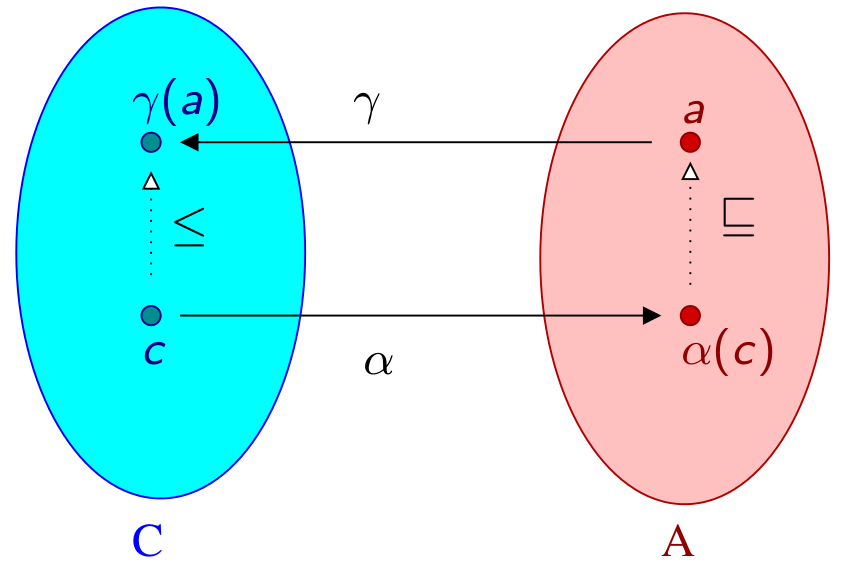
\includegraphics[height=100px]{figures/galois_connection.png}
\end{center}

$\alpha$ is the \textbf{upper adjoint} or \textbf{abstraction}; $A$ is the \textbf{abstract domain}.

$\gamma$ is the \textbf{lower adjoint} or \textbf{concretization}; $C$ is the \textbf{concrete domain}.

\textbf{Properties.} Assume $\forall a, c, \alpha(c) \sqsubseteq a \Leftrightarrow c \leq \gamma (a)$
\begin{enumerate}\setlength{\itemsep}{-0.7mm}
\item $\gamma \circ \alpha$ is \textbf{extensive} : $\forall c, c \leq \gamma (\alpha (c))$
\item $\alpha \circ \gamma$ is \textbf{reductive} : $\forall a, \alpha (\gamma (c)) \sqsubseteq a$
\item $\alpha$ is monotonic
\item $\gamma$ is monotonic
\item $\gamma \circ \alpha \circ \gamma = \gamma$
\item $\alpha \circ \gamma \circ \alpha = \alpha$
\item $\alpha \circ \gamma$ and $\gamma \circ \alpha$ are idempotent
\end{enumerate}

\textbf{Corollary/Definition.} $(\alpha : C \rightarrow A, \gamma : A \rightarrow C)$ is a Galois connection if:
\begin{enumerate}\setlength{\itemsep}{-0.7mm}
\item $\gamma$ is monotonic
\item $\alpha$ is monotonic
\item $\gamma \circ \alpha$ is extensive
\item $\alpha \circ \gamma$ is reductive
\end{enumerate}

\textbf{Corollary.} Given $(C, \leq) \galois{\alpha}{\gamma} (A, \sqsubseteq)$, each adjoint can be \textbf{uniquely defined} in term of the other:
\begin{enumerate}\setlength{\itemsep}{-0.7mm}
\item $\alpha (c) = \sqcap \{ a : c \leq \gamma (a)\} $
\item $\gamma (c) = \vee \{ c : \alpha (c) \sqsubseteq a \} $
\end{enumerate}

\textbf{Corollary.} Given $(C, \leq) \galois{\alpha}{\gamma} (A, \sqsubseteq)$, then
\begin{enumerate}\setlength{\itemsep}{-0.7mm}
\item{$\forall X \subseteq C$, if $\vee X$ exists, then $\alpha (\vee X) = \sqcup \{ \alpha (x) : x \in X\}$}
\item{$\forall X \subseteq C$, if $\sqcap$ exists, then $\gamma (\sqcap) = \wedge \{ \gamma (x): x \in X\}$}
\end{enumerate}

\subsection{Deriving Galois connections}
\textbf{Corollary.} Given $(C, \leq) \galois{\alpha}{\gamma} (A, \sqsubseteq)$ and $(C', \leq') \galois{\alpha}{\gamma} (A', \sqsubseteq')$, we can construct new Galois connections by duality, composition, point-wise lifting by some set $S$, functional lifting of monotonic operators.

\subsection{Galois embeddings}
\textbf{Definition.} If $(C, \leq) \galois{\alpha}{\gamma} (A, \sqsubseteq)$, $(\alpha, \gamma)$ is a \textbf{Galois embedding} $-$ denoted $(C, \leq) \galoiS{\alpha}{\gamma} (A, \sqsubseteq)$ $-$ if it satisfies one of the following properties:
\begin{enumerate}\setlength{\itemsep}{-0.7mm}
\item $\alpha$ is surjective
\item $\gamma$ is injective
\item $\alpha \circ \gamma = id$
\end{enumerate}

%% TODO image 4
\begin{center}
  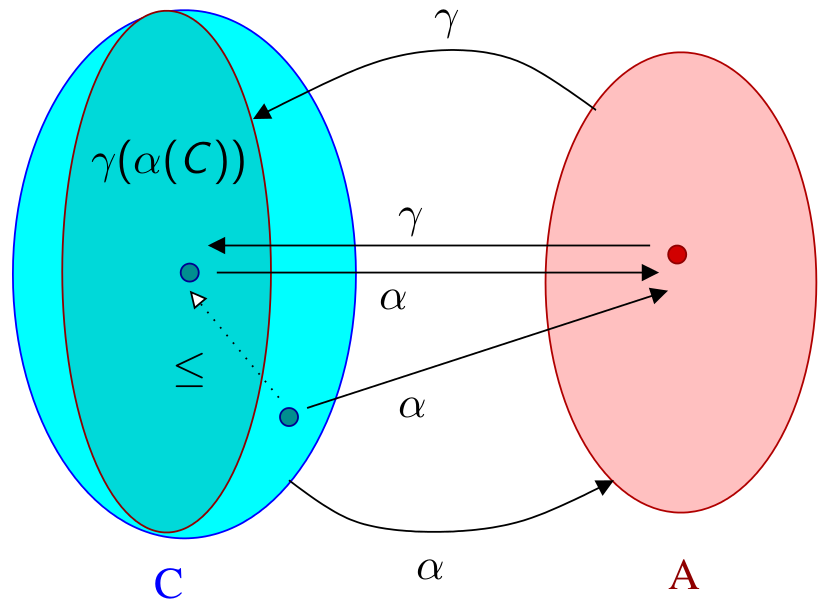
\includegraphics[height=100px]{figures/galois_embedding.png}
\end{center}

\textbf{Corollary.} A Galois conn. can be made into an embedding by \textbf{quotienting} $A$ by the equivalence relation $a \equiv a' \Leftrightarrow \gamma (a) = \gamma (a')$.

\textbf{Definition.} $\rho : X \rightarrow X$ is an \textbf{upper closure} in the poset $(X, \sqsubseteq)$ if it is monotonic, extensive and idempotent.

%% TODO image 5
\begin{center}
  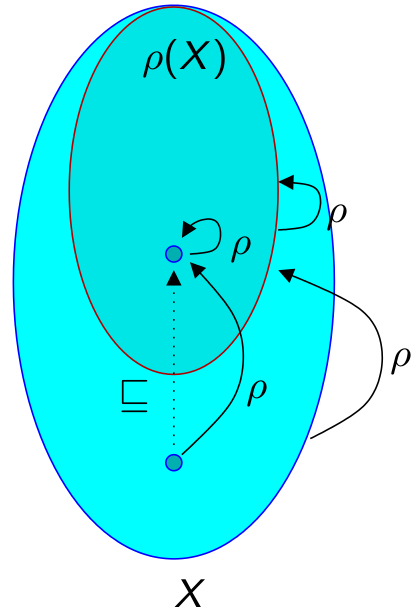
\includegraphics[height=100px]{figures/upper_closure.png}
\end{center}


\textbf{Corollary.} Given $(C, \leq) \galois{\alpha}{\gamma} (A, \sqsubseteq)$, $\gamma \circ \alpha$ is an upper closure on $(C, \leq)$.

\textbf{Corollary.} Given an upper closure $\rho$ on $(X, \sqsubseteq)$, we have $(X, \sqsubseteq) \galois{\rho}{id} (\rho (X), \sqsubseteq)$.

\textbf{Remark.} We can rephrase abstract interpretation using upper closures instead of Galois connections, but we lose : the notion of \textbf{abstract representation} and the ability to have \textbf{several distinct} abstract representations for a single concrete object.

\subsection{Sound, best, and exact abstractions}

\textbf{Definitions.} Given $(C, \leq) \galois{\alpha}{\gamma} (A, \sqsubseteq)$
\begin{itemize}\setlength{\itemsep}{-0.7mm}
\item $a \in A$ is a \textbf{sound abstraction of $c \in C$} if $c \leq \gamma(a)$ or $\alpha (c) \sqsubseteq a$.
\item Given $c \in C$, its \textbf{best abstraction} is $\alpha (c)$
\item $g : A \rightarrow A$ is a \textbf{sound abstraction of $f : C \rightarrow C$} if $\forall a \in A, (f \circ \gamma)(a) \leq (\gamma \circ f)(a)$
\item Given $f : C \overset{\leq}{\rightarrow} C$, its \textbf{best abstraction} is $\alpha \circ f \circ \gamma$
\item $g : A \rightarrow A$ is an \textbf{exact abstraction of $f : C \rightarrow C$} if $f \circ \gamma = \gamma \circ g$
\end{itemize}

\textbf{Corollary.} If $g$ and $g'$ abstract respectively $f$ and $f'$ then
\begin{itemize}\setlength{\itemsep}{-0.7mm}
\item if $f$ and $f'$ are sound abstractions and f is monotonic then $g \circ g'$ is a sound abstraction of $f \circ f'$
\item if $g$, $g'$ are exact abstractions then $g \circ g'$ is an exact abstraction
\item if $g$ and $g'$ are best abstractions, then $g \circ g'$ in \textbf{not} always a best abstraction
\end{itemize}

\textbf{Fixpoint abstraction example theorem.} Let $(C, \leq, \vee, \wedge, \perp, \top)$ be a complete lattice, $g : A \rightarrow A$ a sound abstraction of a monotonic $f : C \overset{\leq}{\rightarrow} C$ and $a$ a postfixpoint of $g$ then $a$ is a sound abstraction of $\operatorname{lfp} f$.

%%%%%%%%%%%%%%%%%%%%%%%%%%%%%%%%%%%%%%%%%%%%%%%%%%%%%%%%%%%%%%%%%%%%%%%%%%%%%%%%%%%%



\rule{0.3\linewidth}{0.25pt}
\scriptsize

Copyright \copyright\ 2012 Winston Chang

http://www.stdout.org/$\sim$winston/latex/


\end{multicols}
\end{document}
